
%{{第二十回}}{第二十回}}

\chapter{王熙凤正言弹妒意\\林黛玉俏语谑娇音}\label{part0024_split_000.htmlux5cux23calibre_pb_0}

{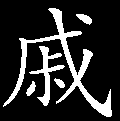
\includegraphics[width=3mm]{../Images/00005}智慧生魔多象,魔生智慧方深。智慧寂灭万缘根,不解智魔作甚。}

话说宝玉在林黛玉房中说``耗子精'',宝钗撞来,讽刺宝玉元宵不知``绿蜡''之典,三人正在房中互相讥刺取笑。那宝玉正恐黛玉饭后贪眠,一时存了食,或夜间走了困,皆非保养身体之法;{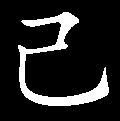
\includegraphics[width=3mm]{../Images/00003}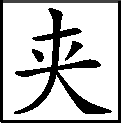
\includegraphics[width=3mm]{../Images/00012}\footnotesize \kaishu 云宝玉亦知医理,却只是在颦、钗等人前方露,亦如后回许多明理之语,只在闺前现露三分,越在雨村等经济人前如痴如呆,实令人可恨。但雨村等视宝玉不是人物,岂知宝玉视彼等更不是人物,故不与接谈也。宝玉之情痴,真乎?假乎?看官细评。}幸而宝钗走来,大家谈笑,那林黛玉方不欲睡,自己才放了心。忽听他房中嚷起来,大家侧耳听了一听,林黛玉先笑道:``这是你妈妈和袭人叫嚷呢。那袭人也罢了,你妈妈再要认真排场他,可见老背晦了。''{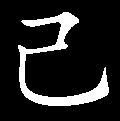
\includegraphics[width=3mm]{../Images/00003}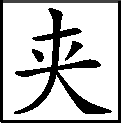
\includegraphics[width=3mm]{../Images/00012}\footnotesize \kaishu 袭卿能使颦卿一赞,愈见彼之为人矣,观者诸公以为如何?}

宝玉忙要赶过来,宝钗忙一把拉住道:{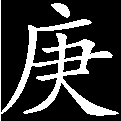
\includegraphics[width=3mm]{../Images/00004}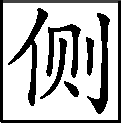
\includegraphics[width=3mm]{../Images/00011}\footnotesize \kaishu 的是宝钗行事。}``你别和你妈妈吵才是,他老糊涂了,倒要让他一步为是。''{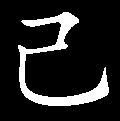
\includegraphics[width=3mm]{../Images/00003}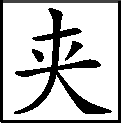
\includegraphics[width=3mm]{../Images/00012}\footnotesize \kaishu 宝钗如何?观者思之。}宝玉道:``我知道了。''说毕走来,只见李嬷嬷拄着拐棍,在当地骂袭人:{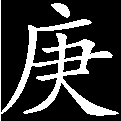
\includegraphics[width=3mm]{../Images/00004}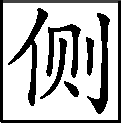
\includegraphics[width=3mm]{../Images/00011}\footnotesize \kaishu 活像过时奶妈骂丫头。}``忘了本的小娼妇!{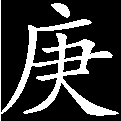
\includegraphics[width=3mm]{../Images/00004}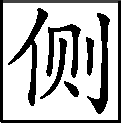
\includegraphics[width=3mm]{../Images/00011}\footnotesize \kaishu 在袭卿身上却叫下撞天屈来。}我抬举起你来,这会子我来了,你大模大样的躺在炕上,见我来也不理一理。一心只想妆狐媚子哄宝玉,{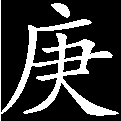
\includegraphics[width=3mm]{../Images/00004}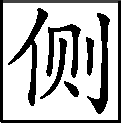
\includegraphics[width=3mm]{../Images/00011}\footnotesize \kaishu 看这句几把批书人吓杀了。}哄的宝玉不理我,听你们的话。{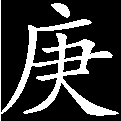
\includegraphics[width=3mm]{../Images/00004}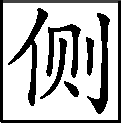
\includegraphics[width=3mm]{../Images/00011}\footnotesize \kaishu 幸有此二句,不然我石兄袭卿扫地矣。}你不过是几两臭银子买来的毛丫头,这屋里你就作耗,如何使得!好不好拉出去配一个小子,{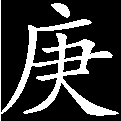
\includegraphics[width=3mm]{../Images/00004}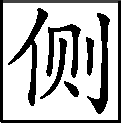
\includegraphics[width=3mm]{../Images/00011}\footnotesize \kaishu 虽写得酷肖,然唐突我袭卿,实难为情。}看你还妖精似的哄宝玉不哄!''{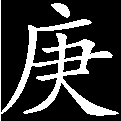
\includegraphics[width=3mm]{../Images/00004}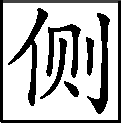
\includegraphics[width=3mm]{../Images/00011}\footnotesize \kaishu 若知``好事多魔'',方会作者之意。}袭人先只道李嬷嬷不过为他躺着生气,少不得分辨说``病了,才出汗,蒙着头,原没看见你老人家''等语。后来只管听他说``哄宝玉''、``妆狐媚'',又说``配小子''等,由不得又愧又委屈,禁不住哭起来。

宝玉虽听了这些话,也不好怎样,少不得替袭人分辨病了吃药等话,又说:``你不信,只问别的丫头们。''李嬷嬷听了这话,益发气起来了,说道:``你只护着那起狐狸,那里认得我了!叫我问谁去?{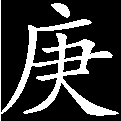
\includegraphics[width=3mm]{../Images/00004}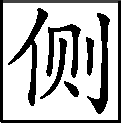
\includegraphics[width=3mm]{../Images/00011}\footnotesize \kaishu 真有是语。}谁不帮着你呢,{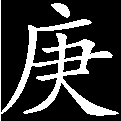
\includegraphics[width=3mm]{../Images/00004}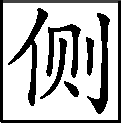
\includegraphics[width=3mm]{../Images/00011}\footnotesize \kaishu 真有是事。}谁不是袭人拿下马来的!{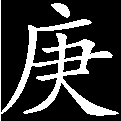
\includegraphics[width=3mm]{../Images/00004}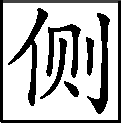
\includegraphics[width=3mm]{../Images/00011}\footnotesize \kaishu 冤枉,冤哉!}我都知道那些事。{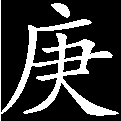
\includegraphics[width=3mm]{../Images/00004}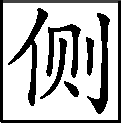
\includegraphics[width=3mm]{../Images/00011}\footnotesize \kaishu 囫囵语,难解。}我只和你在老太太、太太跟前去讲了。把你奶了这么大,{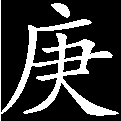
\includegraphics[width=3mm]{../Images/00004}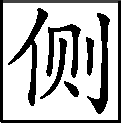
\includegraphics[width=3mm]{../Images/00011}\footnotesize \kaishu 奶妈拿手话。}到如今吃不着奶了,把我丢在一旁,逞着丫头们要我的强。''{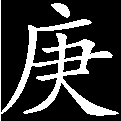
\includegraphics[width=3mm]{../Images/00004}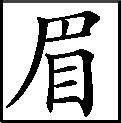
\includegraphics[width=3mm]{../Images/00010}\footnotesize \kaishu 特为乳母传照,暗伏后文倚势奶娘线脉。《石头记》无闲文并虚字在此。壬午孟夏。畸笏老人。}一面说,一面也哭起来。彼时黛玉、宝钗等也走过来劝说:``妈妈你老人家担待他们一点子就完了。''李嬷嬷见他二人{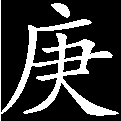
\includegraphics[width=3mm]{../Images/00004}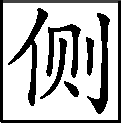
\includegraphics[width=3mm]{../Images/00011}\footnotesize \kaishu 四字,嬷嬷是看重二人身份。}来了,便拉住诉委屈,将当日吃茶,茜雪出去,与昨日酥酪等事,唠唠叨叨说个不清。{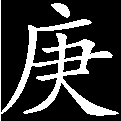
\includegraphics[width=3mm]{../Images/00004}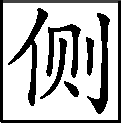
\includegraphics[width=3mm]{../Images/00011}\footnotesize \kaishu 好极,妙极,毕肖极! 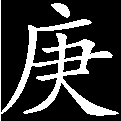
\includegraphics[width=3mm]{../Images/00004}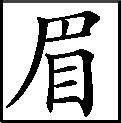
\includegraphics[width=3mm]{../Images/00010}\footnotesize \kaishu 茜雪至``狱神庙''方呈正文。袭人正文标目曰``花袭人有始有终'',余只见有一次誊清时,与``狱神庙慰宝玉''等五六稿,被借阅者迷失,叹叹!丁亥夏。畸笏叟。}

可巧凤姐正在上房算完输赢账,听得后面声嚷动,便知是李嬷嬷老病发了,排揎宝玉的人。------正值他今儿输了钱,{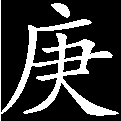
\includegraphics[width=3mm]{../Images/00004}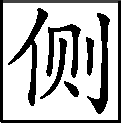
\includegraphics[width=3mm]{../Images/00011}\footnotesize \kaishu 找上文。}迁怒于人。{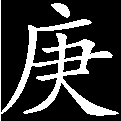
\includegraphics[width=3mm]{../Images/00004}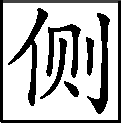
\includegraphics[width=3mm]{../Images/00011}\footnotesize \kaishu 有是争竞事。}便连忙赶过来,拉了李嬷嬷,笑道:``好妈妈,别生气。大节下老太太才喜欢了一日,你是个老人家,别人高声,你还要管他们呢,难道你反不知道规矩,在这里嚷起来,叫老太太生气不成?{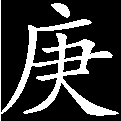
\includegraphics[width=3mm]{../Images/00004}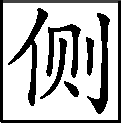
\includegraphics[width=3mm]{../Images/00011}\footnotesize \kaishu 阿凤两提``老太太'',是叫老妪想袭卿是老太太的人,况又双关大体,勿泛泛看去。}你只说谁不好,我替你打他。我家里烧的滚热的野鸡,快来跟我吃酒去。''{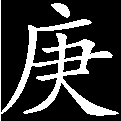
\includegraphics[width=3mm]{../Images/00004}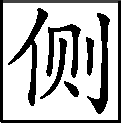
\includegraphics[width=3mm]{../Images/00011}\footnotesize \kaishu 何等现成,何等自然,的是凤卿笔法。}一面说,一面拉着走,又叫:``丰儿,替你李奶奶拿着拐棍子,擦眼泪的手帕子。''{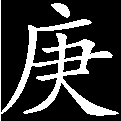
\includegraphics[width=3mm]{../Images/00004}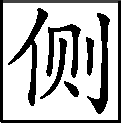
\includegraphics[width=3mm]{../Images/00011}\footnotesize \kaishu 一丝不漏。}那李嬷嬷脚不沾地跟了凤姐走了,一面还说:``我也不要这老命了,越性今儿没了规矩,闹一场子,讨个没脸,强如受那娼妇蹄子的气!''后面宝钗、黛玉随着,见凤姐儿这般,都拍手笑道:``亏这一阵风来,把个老婆子撮了去了。''{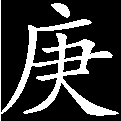
\includegraphics[width=3mm]{../Images/00004}\includegraphics[width=3mm]{../Images/00011}\footnotesize \kaishu 批书人也是这样说。看官将一部书中人一一想来,收拾文字非阿凤俱有琐细引迹事。《石头记》得力处俱在此。}

宝玉点头叹道:``这又不知是那里的账,只拣软的排揎。昨儿又不知是那个姑娘得罪了,上在他账上。''一句未了,晴雯在旁笑道:``谁又不疯了,得罪他作什么。便得罪了他,就有本事承任,不犯着带累别人!''袭人一面哭,一面拉宝玉道:``为我得罪了一个老奶奶,你这会子又为我得罪这些人,这还不够我受的,还只是拉别人。''宝玉见他这般病势,又添了这些烦恼,连忙忍气吞声,安慰他仍旧睡下出汗。又见他汤烧火热,自己守着他,歪在旁边,劝他只养着病,别想着些没要紧的事生气。袭人冷笑道:``要为这些事生气,这屋里一刻还站不得了。{\includegraphics[width=3mm]{../Images/00004}\includegraphics[width=3mm]{../Images/00011}\footnotesize \kaishu 实言,非谬语也。}但只是天长日久,只管这样,可叫人怎么样才好呢?时常我劝你,别为我们得罪人,你只顾一时为我们那样,他们都记在心里,遇着坎儿,说的好说不好听,大家什么意思。''{\includegraphics[width=3mm]{../Images/00004}\includegraphics[width=3mm]{../Images/00011}\footnotesize \kaishu 从``狐媚子''等语来,实实好语,的是袭卿。}一面说,一面禁不住流泪,又怕宝玉烦恼,只得又勉强忍着。{\includegraphics[width=3mm]{../Images/00004}\includegraphics[width=3mm]{../Images/00010}\footnotesize \kaishu 一段特为怡红袭人、晴雯、茜雪三鬟之性情见识身份而写。己卯冬夜。}

一时杂使的老婆子煎了二和药来。宝玉见他才有汗意,不肯叫他起来,自己便端着就枕与他吃了,即令小丫头子们铺炕。袭人道:``你吃饭不吃饭,到底老太太、太太跟前坐一会子,{\includegraphics[width=3mm]{../Images/00004}\includegraphics[width=3mm]{../Images/00011}\footnotesize \kaishu 心中时时刻刻正意语也。}和姑娘们顽一会子再回来。我就静静的躺一躺也好。''宝玉听说,只得替他去了簪环,看他躺下,自往上房来。同贾母吃毕饭,贾母犹欲同那几个老管家嬷嬷斗牌解闷,宝玉记着袭人,便回至房中,见袭人朦朦睡去。自己要睡,天气尚早。彼时晴雯、绮霰、秋纹、碧痕都寻热闹,找鸳鸯、琥珀等耍戏去了,独见麝月一个人在外间房里灯下抹骨牌。宝玉笑问道:``你怎么不同他们顽去?''麝月道:``没有钱。''宝玉道:``床底下堆着那么些,还不够你输的?''麝月道:``都顽去了,这屋里交给谁呢?{\includegraphics[width=3mm]{../Images/00004}\includegraphics[width=3mm]{../Images/00011}\footnotesize \kaishu 正文。}那一个又病了。满屋里上头是灯,地下是火。{\includegraphics[width=3mm]{../Images/00004}\includegraphics[width=3mm]{../Images/00011}\footnotesize \kaishu 灯节。}那些老妈妈子们,老天拔地,伏侍一天,也该叫他们歇歇,小丫头子们也是伏侍了一天,这会子还不叫他们顽顽去。所以让他们都去罢,我在这里看着。''{\includegraphics[width=3mm]{../Images/00004}\includegraphics[width=3mm]{../Images/00010}\footnotesize \kaishu 麝月闲闲无语,令余酸鼻,正所谓对景伤情。丁亥夏。畸笏。}

宝玉听了这话,公然又是一个袭人。{\includegraphics[width=3mm]{../Images/00004}\includegraphics[width=3mm]{../Images/00011}\footnotesize \kaishu 岂敢。}因笑道:``我在这里坐着,你放心去罢。''{\includegraphics[width=3mm]{../Images/00004}\includegraphics[width=3mm]{../Images/00011}\footnotesize \kaishu 每于如此等处,石兄何尝轻轻放过不介意来?亦作者欲瞒看官,又被批书人看出,呵呵。}麝月道:``你既在这里,越发不用去了,咱们两个说话顽笑岂不好?''{\includegraphics[width=3mm]{../Images/00004}\includegraphics[width=3mm]{../Images/00011}\footnotesize \kaishu 全是袭人口气,所以后来代任。}宝玉笑道:``两个作什么呢?怪没意思的,也罢了,早上你说头痒,这会子没什么事,我替你篦头罢。''麝月听了便道:``就是这样。''说着,将文具镜匣搬来,卸去钗钏,打开头发,宝玉拿了篦子替他一一的梳篦。{\includegraphics[width=3mm]{../Images/00004}\includegraphics[width=3mm]{../Images/00011}\footnotesize \kaishu 金闺细事如此写。}只篦了三五下,只见晴雯忙忙走进来取钱。一见了他两个,便冷笑道:``哦,交杯盏还没吃,倒上头了!''{\includegraphics[width=3mm]{../Images/00004}\includegraphics[width=3mm]{../Images/00011}\footnotesize \kaishu 虽谑语,亦少露怡红细事。}宝玉笑道:``你来,我也替你篦一篦。''晴雯道:``我没那么大福。''说着,拿了钱,便摔帘子出去了。

宝玉在麝月身后,麝月对镜,二人在镜内相视。{\includegraphics[width=3mm]{../Images/00004}\includegraphics[width=3mm]{../Images/00011}\footnotesize \kaishu 此系石兄得意处。}宝玉便向镜内笑道:``满屋里就只是他磨牙。''麝月听说,忙向镜中摆手,{\includegraphics[width=3mm]{../Images/00004}\includegraphics[width=3mm]{../Images/00011}\footnotesize \kaishu 好看,趣。}宝玉会意。忽听``唿''一声帘子响,晴雯又跑进来,问道:{\includegraphics[width=3mm]{../Images/00004}\includegraphics[width=3mm]{../Images/00011}\footnotesize \kaishu 麝月摇手为此,可儿可儿!}``我怎么磨牙了?{\includegraphics[width=3mm]{../Images/00004}\includegraphics[width=3mm]{../Images/00011}\footnotesize \kaishu 好看煞!}咱们倒得说说。''{\includegraphics[width=3mm]{../Images/00004}\includegraphics[width=3mm]{../Images/00010}\footnotesize \kaishu 娇憨满纸,令人叫绝。壬午九月。}麝月笑道:``你去你的罢,又来问人了。''晴雯笑道:``你又护着。你们那瞒神弄鬼的,{\includegraphics[width=3mm]{../Images/00004}\includegraphics[width=3mm]{../Images/00011}\footnotesize \kaishu 找上文。}我都知道。等我捞回本儿来再说话。''说着,一径出去了。{\includegraphics[width=3mm]{../Images/00003}\includegraphics[width=3mm]{../Images/00012}\footnotesize \kaishu 闲闲一段儿女口舌,却写麝月一人。{(有)}{[}在{]}袭人出嫁之后,宝玉、宝钗身边还有一人,虽不及袭人周到,亦可免微嫌小弊等患,方不负宝钗之为人也。故袭人出嫁后云``好歹留着麝月''一语,宝玉便依从此话。可见袭人出嫁,虽去实未去也。写晴雯之疑忌,亦为下文跌扇角口等文伏脉,却又轻轻抹去。正见此时都在幼时,虽微露其疑忌,见得人各禀天真之性,善恶不一,往后渐大渐生心矣。但观者凡见晴雯诸人则恶之,何愚也哉!要知自古及今,愈是尤物,其猜忌嫉妒愈甚。若一味浑厚大量涵养,则有何可令人怜爱护惜哉?然后知宝钗、袭人等行为,并非一味蠢拙古板以女夫子自居,当绣幕灯前、绿窗月下,亦颇有或调或妒、轻俏艳丽等说,不过一时取乐买笑耳,非切切一味妒才嫉贤也,是以高诸人百倍。不然,宝玉何甘心受屈于二女夫子哉?看过后文则知矣。故观书诸君子不必恶晴雯,正该感晴雯金闺绣阁中生色方是。}这里宝玉通了头,命麝月悄悄的伏侍他睡下,不肯惊动袭人。一宿无话。

至次日清晨起来,袭人已是夜间发了汗,觉得轻省了些,只吃些米汤静养。宝玉放了心,因饭后走到薛姨妈这边来闲逛。彼时正月内,学房中放年学,闺阁中忌针,却都是闲时。因贾环也过来顽,正遇见宝钗、香菱、莺儿三个赶围棋作耍,贾环见了也要顽。宝钗素习看他亦如宝玉,并没他意,今儿听他要顽,让他上来坐了一处顽。一磊十个钱,头一回自己赢了,心中十分欢喜。{\includegraphics[width=3mm]{../Images/00004}\includegraphics[width=3mm]{../Images/00010}\footnotesize \kaishu 写环兄先赢,亦是天生地设现成文字。己卯冬夜。}后来接连输了几盘,便有些着急。赶着这盘正该自己掷骰子,若掷个七点便赢,若掷个六点,下该莺儿掷三点就赢了。因拿起骰子来,狠命一掷,一个作定了五,那一个乱转。莺儿拍着手只叫``幺'',{{
}\includegraphics[width=3mm]{../Images/00003}\includegraphics[width=3mm]{../Images/00012}\footnotesize \kaishu 娇憨如此。 {\includegraphics[width=3mm]{../Images/00004}\includegraphics[width=3mm]{../Images/00011}\footnotesize \kaishu 好看煞。}}贾环便瞪着眼,``六------七------八''混叫。那骰子偏生转出幺来。贾环急了,伸手便抓起骰子来,然后就拿钱,{\includegraphics[width=3mm]{../Images/00004}\includegraphics[width=3mm]{../Images/00011}\footnotesize \kaishu 更也好看。}说是个六点。莺儿便说:``分明是个幺!''宝钗见贾环急了,便瞅莺儿说道:``越大越没规矩,难道爷们还赖你?{\includegraphics[width=3mm]{../Images/00006}\includegraphics[width=3mm]{../Images/00011}\footnotesize \kaishu 酷肖。}还不放下钱来呢!''莺儿满心委屈,见宝钗说,不敢则声,只得放下钱来,口内嘟囔说:``一个作爷的,还赖我们这几个钱,{\includegraphics[width=3mm]{../Images/00004}\includegraphics[width=3mm]{../Images/00011}\footnotesize \kaishu 酷肖。}连我也不放在眼里。前儿和宝玉顽,他输了那些,也没着急。{\includegraphics[width=3mm]{../Images/00004}\includegraphics[width=3mm]{../Images/00011}\footnotesize \kaishu 倒卷帘法,实写幼时往事。可伤。}下剩的钱,还是几个小丫头子们一抢,他一笑就罢了。''宝钗不等说完,连忙断喝。贾环道:``我拿什么比宝玉呢。你们怕他,都和他好,{\includegraphics[width=3mm]{../Images/00004}\includegraphics[width=3mm]{../Images/00011}\footnotesize \kaishu 蠢驴!}都欺负我不是太太养的。''{\includegraphics[width=3mm]{../Images/00004}\includegraphics[width=3mm]{../Images/00011}\footnotesize \kaishu 观者至此,有不卷帘厌看者乎?余替宝卿实难为情。}说着,便哭了。宝钗忙劝他:``好兄弟,快别说这话,人家笑话你。''又骂莺儿。

正值宝玉走来,见了这般形况,问是怎么了。贾环不敢则声。宝钗素知他家规矩,凡作兄弟的,都怕哥哥,{\includegraphics[width=3mm]{../Images/00003}\includegraphics[width=3mm]{../Images/00012}\footnotesize \kaishu 大族规矩原是如此,一丝儿不错。}却不知那宝玉是不要人怕他的。他想着:``兄弟们一并都有父母教训,何必我多事,反生疏了。况且我是正出,他是庶出,饶这样还有人背后谈论,{\includegraphics[width=3mm]{../Images/00004}\includegraphics[width=3mm]{../Images/00011}\footnotesize \kaishu 此意不呆。}还禁得辖治他了。''更有个呆意思存在心里。{{\includegraphics[width=3mm]{../Images/00004}\includegraphics[width=3mm]{../Images/00010}\footnotesize \kaishu 又用讳人语瞒着看官。己卯冬{(辰)}{[}夜{]}。}}------你道是何呆意?因他自幼姊妹丛中长大,亲姊妹有元春、探春,伯叔的有迎春、惜春,亲戚中又有史湘云、林黛玉、薛宝钗等诸人。他便料定,原来天生人为万物之灵,凡山川日月之精秀,只钟于女儿,须眉男子不过是些渣滓浊沫而已。因有这个呆念在心,把一切男子都看成混沌浊物,可有可无。只是父亲叔伯兄弟中,因孔子是亘古第一人说下的,不可忤慢,只得要听他这句话。{\includegraphics[width=3mm]{../Images/00004}\includegraphics[width=3mm]{../Images/00011}\footnotesize \kaishu 听了这一个人之话,岂是呆子?由你自己说罢。我把你作极乖的人看。}所以,弟兄之间不过尽其大概的情理就罢了,并不想自己是丈夫,须要为子弟之表率。是以贾环等都不怕他,却怕贾母,才让他三分。如今宝钗恐怕宝玉教训他,倒没意思,便连忙替贾环掩饰。宝玉道:``大正月里哭什么?这里不好,你别处顽去。你天天念书,倒念糊涂了。比如这件东西不好,横竖那一件好,就弃了这件取那个。难道你守着这个东西哭一会子就好了不成?你原是来取乐顽的,既不能取乐,就往别处去寻乐顽去。哭一会子,难道算取乐顽了不成?倒招自己烦恼,不如快去为是。''{\includegraphics[width=3mm]{../Images/00004}\includegraphics[width=3mm]{../Images/00011}\footnotesize \kaishu 呆子都会立这样意,说这样话?}贾环听了,只得回来。

赵姨娘见他这般,因问:``又是那里垫了踹窝来了?''{\includegraphics[width=3mm]{../Images/00004}\includegraphics[width=3mm]{../Images/00011}\footnotesize \kaishu 多事人等口{[}角{]}谈吐。}一问不答,{\includegraphics[width=3mm]{../Images/00004}\includegraphics[width=3mm]{../Images/00011}\footnotesize \kaishu 毕肖。}再问时,贾环便说:``同宝姐姐顽的,莺儿欺负我,赖我的钱,宝玉哥哥撵我来了。''赵姨娘啐道:``谁叫你上高抬攀去了?\href{../Text/part0024_split_000.html\#lnkback_1_a}{\textsuperscript{①}}下流没脸的东西!那里顽不得?谁叫你跑了去讨没意思!''

正说着,可巧凤姐在窗外过,都听在耳内,便隔窗说道:``大正月又怎么了?环兄弟小孩子家,一半点儿错了,你只教导他,说这些淡话作什么!凭他怎么去,还有太太老爷管他呢,就大口啐他!{\includegraphics[width=3mm]{../Images/00004}\includegraphics[width=3mm]{../Images/00011}\footnotesize \kaishu 反得了理了,所谓贬中褒,想赵姨即不畏阿凤,亦无可回答。}他现是主子,不好了,横竖有教导他的人,与你什么相干!环兄弟,出来,跟我顽去。''{\includegraphics[width=3mm]{../Images/00004}\includegraphics[width=3mm]{../Images/00010}\footnotesize \kaishu 嫡嫡是彼亲生,句句竟成正中贬,赵姨实难答言。至此方知题标用``弹''字甚妥协。己卯冬夜。}贾环素日怕凤姐比怕王夫人更甚,听见叫他,忙唯唯的出来。赵姨娘也不敢则声。{\includegraphics[width=3mm]{../Images/00004}\includegraphics[width=3mm]{../Images/00011}\footnotesize \kaishu ``弹妒意''正文。}凤姐向贾环道:``你也是个没气性的!时常说给你:要吃,要喝,要顽,要笑,只爱同那一个姐姐妹妹哥哥嫂子顽,就同那个顽。你不听我的话,反叫这些人教的歪心邪意,{\includegraphics[width=3mm]{../Images/00004}\includegraphics[width=3mm]{../Images/00011}\footnotesize \kaishu 借人发脱,好阿凤!好口齿!句句正言正理。赵姨安得不抿翅低头,静听发挥?批至此,不禁一大白又{[}一{]}大白矣!}狐媚子霸道的。自己不尊重,要往下流走,安着坏心,还只管怨人家偏心。输了几个钱?{\includegraphics[width=3mm]{../Images/00004}\includegraphics[width=3mm]{../Images/00011}\footnotesize \kaishu 转得好。}就这么个样儿!''贾环见问,只得诺诺的回说:``输了一二百。''凤姐道:``亏你还是爷,输了一二百钱就这样!''{{\includegraphics[width=3mm]{../Images/00004}\includegraphics[width=3mm]{../Images/00011}\footnotesize \kaishu 作者{(当)}{[}尚{]}记一大百乎?{(笑笑)}{[}叹叹{]}。}}回头叫丰儿:``去取一吊钱来,姑娘们都在后头顽呢,把他送了顽去。{\includegraphics[width=3mm]{../Images/00004}\includegraphics[width=3mm]{../Images/00011}\footnotesize \kaishu 收拾得好。}你明儿再这么下流狐媚子,我先打了你,打发人告诉学里,皮不揭了你的!为你这个不尊重,{\includegraphics[width=3mm]{../Images/00004}\includegraphics[width=3mm]{../Images/00011}\footnotesize \kaishu 又一折笔,更觉有味。}恨的你哥哥牙痒,不是我拦着,窝心脚把你的肠子窝出来了。''喝命:``去罢!''{\includegraphics[width=3mm]{../Images/00004}\includegraphics[width=3mm]{../Images/00011}\footnotesize \kaishu 本来面目,断不可少。}贾环诺诺的跟了丰儿,得了钱,{\includegraphics[width=3mm]{../Images/00004}\includegraphics[width=3mm]{../Images/00011}\footnotesize \kaishu 三字写着环哥。}自己和迎春等顽去。不在话下。{\includegraphics[width=3mm]{../Images/00003}\includegraphics[width=3mm]{../Images/00012}\footnotesize \kaishu 一段大家子奴妾吆吻,如见如闻,正为下文五鬼作引也。余谓宝玉肯效凤姐一点馀风,亦可继荣、宁之盛,诸公当为如何?}

且说宝玉正和宝钗顽笑,忽见人说:``史大姑娘来了。''{\includegraphics[width=3mm]{../Images/00003}\includegraphics[width=3mm]{../Images/00012}\footnotesize \kaishu 妙极!凡宝玉、宝钗正闲相遇时,非黛玉来,即湘云来,是恐泄漏文章之精华也。若不如此,则宝玉久坐忘情,必被宝卿见弃,杜绝后文成其夫妇时无可谈旧之情,有何趣味哉?}宝玉听了,抬身就走。宝钗笑道:``等着,{\includegraphics[width=3mm]{../Images/00004}\includegraphics[width=3mm]{../Images/00010}\footnotesize \kaishu ``等着''二字大有神情。看官闭目熟思,方知趣味。非批书人漫拟也。己卯冬夜。}咱们两个一齐走,瞧瞧他去。''说着,下了炕,同宝玉一齐来至贾母这边。只见史湘云大笑大说的,见他两个来,忙问好厮见。{\includegraphics[width=3mm]{../Images/00003}\includegraphics[width=3mm]{../Images/00012}\footnotesize \kaishu 写湘云又一笔法,特犯不犯。}正值林黛玉在旁,因问宝玉:``在那里的?''宝玉便说:``在宝姐姐家的。''黛玉冷笑道:``我说呢,亏在那里绊住,不然早就飞了来了。''{\includegraphics[width=3mm]{../Images/00004}\includegraphics[width=3mm]{../Images/00011}\footnotesize \kaishu 总是心中事语,故机括一动,随机而出。}宝玉笑道:``只许同你顽,替你解闷儿。不过偶然去他那里一趟,就说这话。''林黛玉道:``好没意思的话!去不去管我什么事,我又没叫你替我解闷儿。可许你从此不理我呢!''说着,便赌气回房去了。

宝玉忙跟了来,问道:``好好的又生气了?就是我说错了,你到底也还坐在那里,和别人说笑一会子。又来自己纳闷。''林黛玉道:``你管我呢!''宝玉笑道:``我自然不敢管你,只没有个看着你自己作践了身子呢。''林黛玉道:``我作践坏了身子,我死,与你何干!''宝玉道:``何苦来,大正月里,死了活了的。''林黛玉道:``偏说死!我这会子就死!你怕死,你长命百岁的,如何?''宝玉笑道:``要像只管这样闹,我还怕死呢?倒不如死了干净。''黛玉忙道:``正是了,要是这样闹,不如死了干净。''宝玉道:``我说我自己死了干净,别听错了话赖人。''正说着,宝钗走来道:``史大妹妹等你呢。''说着,便推宝玉走了。{\includegraphics[width=3mm]{../Images/00003}\includegraphics[width=3mm]{../Images/00012}\footnotesize \kaishu 此时宝钗尚未知他二人心性,故来劝;后文察其心性,故掷之不闻矣。}这里林黛玉越发气闷,只向窗前流泪。没两盏茶的工夫,宝玉仍来了。{\includegraphics[width=3mm]{../Images/00003}\includegraphics[width=3mm]{../Images/00012}\footnotesize \kaishu 盖宝玉亦是心中只有黛玉,见宝钗难却其意,故暂随彼去,以完宝钗之情,故少坐仍来也。}林黛玉见了,越发抽抽噎噎的哭个不住。宝玉见了这样,知难挽回,打叠起千百样的款语温言来劝慰。不料自己未张口,{\includegraphics[width=3mm]{../Images/00004}\includegraphics[width=3mm]{../Images/00011}\footnotesize \kaishu 石头惯用如此笔仗。}只见黛玉先说道:``你又来作什么?横竖如今有人和你顽,比我又会念,又会作,又会写,又会说笑,又怕你生气拉了你去,你又作什么来?死活凭我去罢了!''宝玉听了忙上来悄悄的说道:``你这么个明白人,难道连`亲不间疏,先不僭后'{\includegraphics[width=3mm]{../Images/00004}\includegraphics[width=3mm]{../Images/00011}\footnotesize \kaishu 八字足可消气。}也不知道?我虽糊涂,却明白这两句话。头一件,咱们是姑舅姊妹,宝姐姐是两姨姊妹,论亲戚,他比你疏。第二件,你先来,咱们两个一桌吃,一床睡,长的这么大了,他是才来的,岂有个为他疏你的?''林黛玉啐道:``我难道为叫你疏他?我成了个什么人了呢!我为的是我的心。''宝玉道:``我也为的是你的心。难道你就知你的心,不知我的心不成?''{\includegraphics[width=3mm]{../Images/00003}\includegraphics[width=3mm]{../Images/00012}\footnotesize \kaishu 此二语不独观者不解,料作者亦未必解;不但作者未必解,想石头亦不解,不过述宝、林二人之语耳。石头既未必解,宝、林此刻更自己亦不解,皆随口说出耳。若观者必欲要解,须自揣自身是宝、林之流,则洞然可解;若自料不是宝、林之流,则不必求解矣。万不可{(记)}{[}借{]}此二句不解,错谤宝、林及石头、作者等人。}林黛玉听了,低头一语不发,半日说道:``你只怨人行动嗔怪了你,你再不知道你自己怄人难受。就拿今日天气比,分明今儿冷的这样,你怎么倒反把个青肷披风脱了呢?''{\includegraphics[width=3mm]{../Images/00003}\includegraphics[width=3mm]{../Images/00012}\footnotesize \kaishu 真真奇绝妙文,真如羚羊挂角,无迹可求。此等奇妙,非口中笔下可形容出者。}宝玉笑道:``何尝不穿着,见你一恼,我一炮燥就脱了。''黛玉叹道:``回来伤了风,又该饿着吵吃的了。''{\includegraphics[width=3mm]{../Images/00003}\includegraphics[width=3mm]{../Images/00012}\footnotesize \kaishu 一语仍归儿女本传,却又轻轻抹去也。 {\includegraphics[width=3mm]{../Images/00004}\includegraphics[width=3mm]{../Images/00010}\footnotesize \kaishu 明明写湘云来是正文,只用二三答言,反接写玉、林小角口,又用宝钗岔开,仍不了局。再用千句柔言百般温态,正在情完未完之时,湘云突至,``谑娇音''之文才见。真正``卖弄有家私''}}\href{../Text/part0024_split_000.html\#lnkback_2_a}{\textsuperscript{②}}{之笔也。丁亥夏。畸笏叟。}

二人正说着,只见湘云走来,笑道:``二哥哥,林姐姐,你们天天一处顽,我好容易来了,也不理我一理儿。''林黛玉笑道:``偏是咬舌子爱说话,连个`二'哥哥也叫不出来,只是`爱'哥哥`爱'哥哥的。回来赶围棋儿,又该你闹`幺爱三四五'了。''宝玉笑道:``你学惯了他,明儿连你还咬起来呢。''{\includegraphics[width=3mm]{../Images/00003}\includegraphics[width=3mm]{../Images/00012}\footnotesize \kaishu 可笑近之野史中,满纸羞花闭月、莺啼燕语。殊不知真正美人方有一陋处,如太真之肥、飞燕之瘦、西子之病,若施于别个,不美矣。今见``咬舌''二字加之湘云,是何大法手眼敢用此二字哉?不独不见其陋,且更觉轻俏娇媚,俨然一娇憨湘云立于纸上,掩卷合目思之,其``爱''``厄''娇音如入耳内。然后将满纸莺啼燕语之字样填粪窖可也。}史湘云道:``他再不放人一点儿,专挑人的不好。你自己便比世人好,也不犯着见一个打趣一个。指出一个人来,你敢挑他,我就伏你。''黛玉忙问是谁。湘云道:``你敢挑宝姐姐的短处,就算你是好的。我算不如你,他怎么不及你呢。''林黛玉听了,冷笑道:``我当是谁,原来是他!我那里敢挑他呢。''{\includegraphics[width=3mm]{../Images/00004}\includegraphics[width=3mm]{../Images/00010}\footnotesize \kaishu 此作者放笔写,非褒钗贬颦也。己卯冬夜。}宝玉不等说完,忙用话岔开。湘云笑道:``这一辈子我自然比不上你。我只保佑着明儿得一个咬舌的林姐夫,时时刻刻你可听`爱'`厄'去。阿弥陀佛,那才现在我眼里!''说的众人一笑,湘云忙回身跑了。要知端详,下回分解。

{\includegraphics[width=3mm]{../Images/00003}此回文字重作轻抹。得力处是凤姐拉李嬷嬷去,借环哥弹压赵姨。细致处宝钗为李嬷劝宝玉,安慰环哥,断喝莺儿。至急为难处是宝、颦论心。无可奈何处是``就拿今日天气比'',``黛玉冷笑道:`我当谁,原来是他!'''冷眼最好看处是宝钗、黛玉看凤姐拉李嬷云``这一阵风'';玉、麝一节;湘云到,宝玉就走,宝钗笑说``等着'';湘云大笑大说;颦儿学咬舌;湘云念佛跑了\ldots{}\ldots{}数节,可使看官于纸上能耳闻目睹其音其形之文。}

{\href{../Text/part0024_split_000.html\#navto_1_a}{①}``高抬攀'',下文第二十五回又作``高台板'',或当作``高台盘''。}

{\href{../Text/part0024_split_000.html\#navto_2_a}{②}``卖''原误``费'',参俞平伯辑评本改。``卖弄有家私'':语出元王实甫《西厢记》第三本第一折:``哎,你个馋穷酸俫没意儿,卖弄你有家私,莫不图谋你东西来到此?''}
